\section{CÔNG NGHỆ HIỆN THỰC}
\subsection{TSVector}
\subsubsection{Tổng quan}
\hspace*{1cm} TSvector là một kiểu dữ liệu trong PostgreSQL được sử dụng để lưu trữ các từ khóa được tối ưu hóa cho tìm kiếm toàn văn bản (FTS). Nó được tạo ra từ một chuỗi văn bản, nơi chuỗi văn bản đó được phân tích thành các từ khóa, loại bỏ các từ dừng (stop words) và sau đó sắp xếp theo thứ tự từ điển.
\subsubsection{Các tính năng nổi bật}
TSVector được sử dụng khá phổ biến nhờ vào các tính năng như sau:
\begin{itemize}
    \item Tìm kiếm toàn văn bản: TSvector cho phép tìm kiếm toàn bộ văn bản trong một cột, thay vì chỉ tìm kiếm các từ khóa khớp chính xác. Thông qua đó giúp tìm thấy các tài liệu có liên quan đến truy vấn , ngay cả khi chúng không chứa tất cả các từ khóa chính xác đã tìm kiếm.
    \item Hỗ trợ nhiều ngôn ngữ: TSvector hỗ trợ nhiều ngôn ngữ khác nhau, bao gồm tiếng Việt. Điều này giúp người dùng có thể tìm kiếm văn bản bằng ngôn ngữ mà người đó thông thạo , hiểu sâu nhất.
    \item Hỗ trợ nhiều loại truy vấn: TSvector hỗ trợ nhiều loại truy vấn khác nhau, bao gồm truy vấn AND, OR, NOT, gần đúng và truy vấn theo tiền tố. Hỗ trợ tìm kiếm văn bản một cách linh hoạt hơn.
\end{itemize}
\begin{figure}[H]
    \centering
    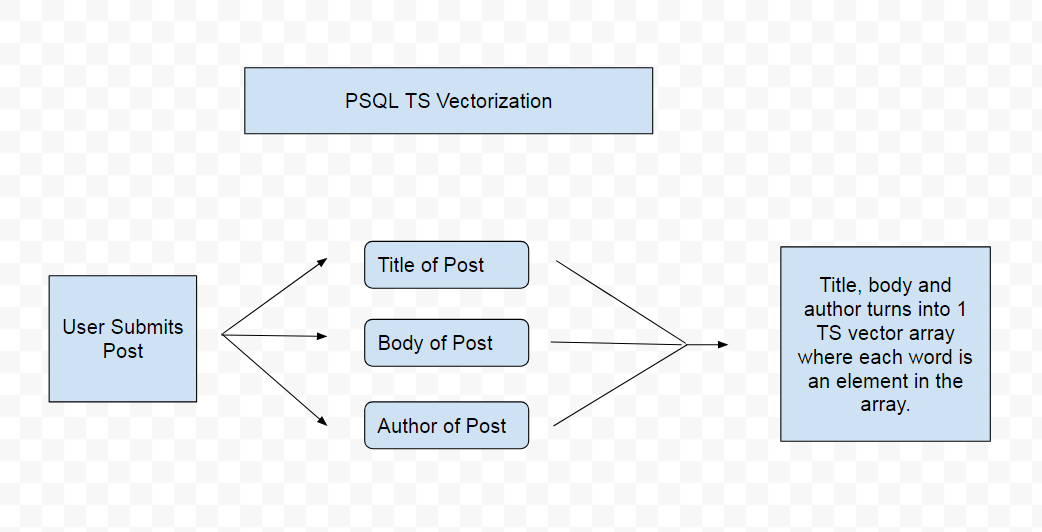
\includegraphics[width=0.8\textwidth]{Images/technology/TSVector.png}
    \caption{Nguyên lí hoạt động của TSVector}
\end{figure}
\subsubsection{Phân tích ưu và nhược điểm}
\textbf{Ưu điểm}
\begin{itemize}
    \item Tăng tốc độ tìm kiếm: TSvector sử dụng các kỹ thuật lập chỉ mục để tăng tốc độ tìm kiếm. Do vậy có thể tìm thấy kết quả nhanh hơn, ngay cả khi đang tìm kiếm trong một tập dữ liệu lớn.
    \item Sử dụng từ đồng nghĩa: TSvector có thể sử dụng từ đồng nghĩa bằng cách khai báo để tìm kiếm các tài liệu có chứa các từ khóa tương tự như truy vấn.
    \item Phân tích cú pháp: TSvector có thể phân tích cú pháp văn bản để hiểu rõ hơn về ý nghĩa của nó.
\end{itemize}
\textbf{Nhược điểm}
\begin{itemize}
    \item Khá tốn kém: cần phải có một tập dữ liệu lớn để sử dụng cho TSvector. Điều này là do TSvector sử dụng các kỹ thuật lập chỉ mục để tăng tốc độ tìm kiếm, mà các kỹ thuật lập chỉ mục này có thể tốn nhiều dung lượng lưu trữ.
    \item Độ phức tạp cao : Có thể có độ phức tạp cao khi sử dụng nếu bạn cần thực hiện các truy vấn phức tạp, do TSvector hỗ trợ nhiều loại truy vấn khác nhau, và mỗi loại truy vấn có cú pháp riêng.
    \item Kết quả không có độ chính xác cao : kết quả không chính xác nếu có một tập dữ liệu có chất lượng kém. TSVector hoạt động dựa vào các kỹ thuật lập chỉ mục để tìm kiếm, mà các kỹ thuật lập chỉ mục này có thể không chính xác nếu văn bản trong tập dữ liệu bị lỗi hoặc không chính xác.
\end{itemize}
\subsection{PgVector}
\subsubsection{Tổng quan}
Pgvector là một thư viện mở rộng dựa trên PostgreSQL nhằm cung cấp các chức năng mạnh mẽ để làm việc với vectơ trong không gian đa chiều, đồng thời giới thiệu một kiểu dữ liệu chuyên dụng, toán tử và hàm cho phép lưu trữ, thao tác và phân tích dữ liệu vectơ hiệu quả trực tiếp trong cơ sở dữ liệu PostgreSQL.
\subsubsection{Các tính năng nổi bật}
\begin{itemize}
    \item Lưu trữ vectơ: cung cấp một kiểu dữ liệu mới để lưu trữ vectơ trong PostgreSQL. Loại dữ liệu này được tối ưu hóa để lưu trữ vectơ hiệu quả và có thể được sử dụng để lưu trữ các vectơ có độ dài khác nhau.
    \item Thao tác vectơ: bao gồm một loạt các toán tử và hàm cho phép thao tác vectơ, chẳng hạn như cộng, trừ, nhân và chia. Các toán tử và hàm được tối ưu hóa để thực hiện hiệu quả và có thể được sử dụng để thực hiện các phép tính vectơ phức tạp.
    \item Phân tích vectơ: tích hợp một số hàm cho phép phân tích dữ liệu vectơ, chẳng hạn như tính toán độ dài vectơ, tính toán khoảng cách giữa hai vectơ và tìm kiếm những dữ liệu có liên quan nhất. Các hàm có thể được sử dụng để thực hiện các tác vụ như tìm kiếm tương tự, nhóm dữ liệu và giảm kích thước.
\end{itemize}
\subsubsection{Phân tích ưu và nhược điểm}
\textbf{Ưu điểm}
\begin{itemize}
    \item Hiệu suất : pgvector được tối ưu hóa để lưu trữ, thao tác và phân tích dữ liệu vectơ một cách hiệu quả. Điều này làm cho nó trở thành lựa chọn lý tưởng cho các ứng dụng cần xử lý lượng lớn dữ liệu vectơ 
    \item Tính linh hoạt :  hỗ trợ lưu trữ và phân tích nhiều loại vectơ khác nhau, bao gồm vectơ văn bản, vectơ hình ảnh, vectơ âm thanh và vectơ dữ liệu cảm biến
    \item Dễ sử dụng : Các hàm và toán tử được thiết kế rõ ràng và dễ hiểu, cho phép người dùng thực hiện các thao tác vectơ phức tạp một cách hiệu quả.
\end{itemize}
\textbf{Nhược điểm}
\begin{itemize}
    \item Khả năng tương thích : mặc dù pgvector là một phần mở rộng phổ biến, nó vẫn có thể chưa được hỗ trợ đầy đủ bởi tất cả các công cụ và thư viện PostgreSQL.
    \item Độ phức tạp : so với các phương pháp lưu trữ dữ liệu truyền thống, pgvector có thể có độ phức tạp cao hơn về mặt triển khai và sử dụng.
\end{itemize}
\subsection{React Native}
\subsubsection{Tổng quan}
\hspace*{1cm} React Native là một framework để xây dựng các ứng dụng di động cho cả hai hệ điều hành iOS và Android sử dụng JavaScript và React. Nó cho phép lập trình viên sử dụng cùng một code base để xây dựng các ứng dụng di động trên nhiều nền tảng mà không cần phải tạo ra hai mã nguồn riêng biệt cho mỗi nền tảng. Điều này giúp cho việc phát triển và bảo trì các ứng dụng di động trở nên dễ dàng hơn và hiệu quả hơn \cite{rn}.
\subsubsection{Các tính năng nổi bật}
Có nhiều lý do tại sao React Native đang trở thành xu hướng trong việc phát triển các ứng dụng di động. Trong số đó là:
\begin{itemize}
    \item[-] Sử dụng JavaScript: React Native cho phép phát triển các ứng dụng di động sử dụng JavaScript, một ngôn ngữ lập trình rất phổ biến và được sử dụng rộng rãi trong cộng đồng lập trình viên.
    \item[-] Mã nguồn chung: React Native cho phép sử dụng một mã nguồn chung cho cả hai hệ điều hành iOS và Android, giúp giảm thời gian và chi phí phát triển và bảo trì.
    \item[-] Tốc độ phát triển nhanh: React Native cung cấp môi trường phát triển nhanh và dễ dàng cho phép nhanh chóng xây dựng và thử nghiệm các tính năng mới.
    \item[-] Tốt cho UX: React Native cho phép tạo ra các giao diện người dùng tốt và tự nhiên, giúp tăng trải nghiệm người dùng với ứng dụng.
\end{itemize}
\subsubsection{Phân tích ưu và nhược điểm}
\textbf{Ưu điểm}
\begin{itemize}
    \item Khả năng tái sử dụng lại mã nguồn cao, lên đến hơn 90\% cho cả hai nền tảng Android và Ios 
    \item Cộng đồng sử dụng lớn do vậy nên hầu như các vấn đề trục trặc đều có thể tìm kiếm và có được sự giúp đỡ hỗ trọ từ cộng động các nhà phát triển
    \item Có nhiều thư viện hỗ trợ đi kèm, dẽ dàng cho việc nâng cấp phát triển ứng dụng theo ý muốn của nhà phát triển.
    \item Được hỗ trợ và cập nhật liên tục từ Facebook, nhờ đó React Native luôn có thể bắt kịp xu hướng phát triển của điện thoại đông minh
\end{itemize}
\textbf{Nhược điểm}
\begin{itemize}
    \item Do mã nguồn sử dụng cùng lúc cho hai nền tảng Android và Ios nên có thêm lớp abstract layer bên dưới để hỗ trợ cho từng nền tảng vì vậy sẽ chạy không hiệu quả bằng các ngôn ngữ chỉ hỗ trợ 1 nền tảng như kotlin , swift
    \item Quản lý bộ nhớ không hiệu quả cho các ứng dụng đòi hỏi tính toán nhiều
\end{itemize}
\subsection{Node.js}
\subsubsection{Tổng quan}
\hspace*{1cm} Node.js là một môi trường thực thi JavaScript mã nguồn mở, có thể chạy trên nhiều nền tảng như Window, Linux, macOS,...Node.js chạy trên V8 JavaScript Engine, và thực thi mã JavaScript bên ngoài trình duyệt web. Node.js được ra đời vào năm 2009, trước đây được quản lý bởi Node.js Foundation, nhưng hiện đã hợp nhất với JS Foundation thành OpenJS Foundation. Node.js cho phép các nhà phát triển sử dụng JavaScript để viết mã bên phía máy chủ. Khả năng chạy mã JavaScript trên máy chủ thường được sử dụng để tạo nội dung trang web động trước khi trang được gửi tới trình duyệt web của người dùng \cite{nodejs}
\begin{figure}[H]
    \centering
    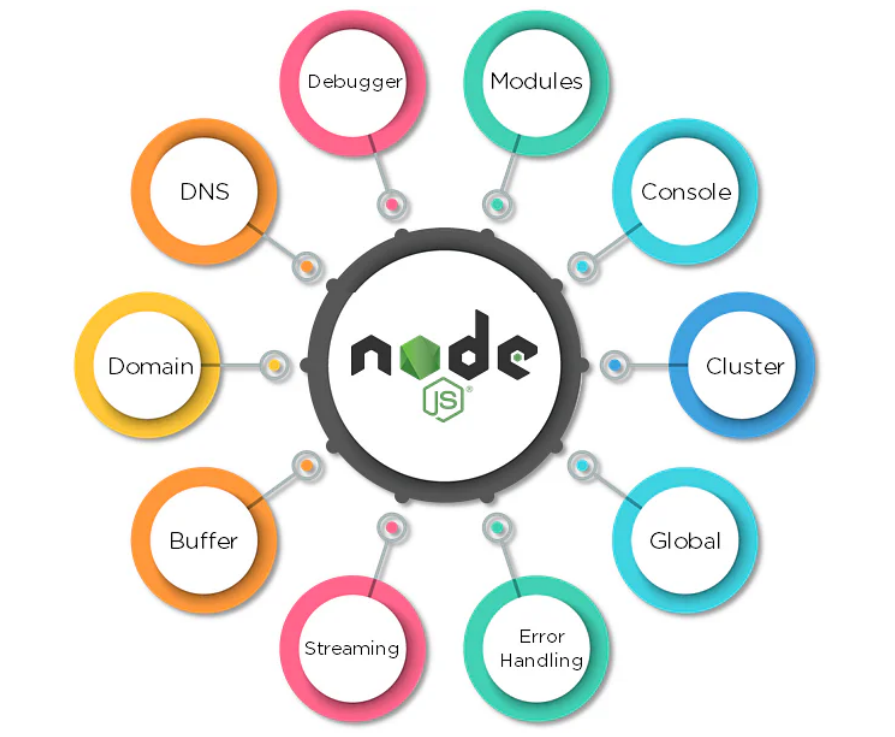
\includegraphics[width=0.6\textwidth]{Images/technology/nodejs-structure.png}
    \caption{Các thành phần nổi bật của NodeJS}
\end{figure}
\subsubsection{Các tính năng nổi bật}
\begin{itemize}
    \item Node.js cho phép chạy mã JavaScript trực tiếp trên máy chủ, cung cấp sự đồng nhất giữa phía máy khách và phía máy chủ trong ứng dụng web.
    \item Mô hình không đồng bộ của Node.js giúp xử lý hàng loạt yêu cầu mà không chờ đợi kết quả của mỗi yêu cầu trước khi bắt đầu yêu cầu tiếp theo, tối ưu cho ứng dụng có nhiều I/O.
    \item Node.js sử dụng mô hình sự kiện để xử lý nhiều yêu cầu mà không cần tạo ra một luồng mới cho mỗi yêu cầu, giúp giảm áp lực lên hệ thống.
    \item Node.js sử dụng hệ thống module để tổ chức mã nguồn, giúp tách biệt chức năng và tái sử dụng mã.
\end{itemize}
\subsubsection{Phân tích ưu và nhược điểm}
\textbf{Ưu điểm}
\begin{itemize}
    \item Có thể xử lý nhiều yêu cầu đồng thời nhờ I/O hướng sự kiện bất đồng bộ.
    \item Đáp ứng được những yêu cầu về thời gian thực.
    \item Chia sẻ cùng một đoạn mã với cả phía máy chủ và máy khách.
    \item Có tốc độ thực thi rất nhanh, đáp ứng được nhu cầu sử dụng của khách truy cập "khổng lồ" trong thời gian ngắn.
    \item Có một cộng đồng sử dụng rộng lớn và hoạt động tích cực, nhiều đoạn mã được chia sẻ giúp đỡ lẫn nhau.
\end{itemize}
\textbf{Nhược điểm}
\begin{itemize}
    \item NodeJS không phù hợp với các tác vụ đòi hỏi nhiều CPU hay các tác vụ tính toán phức tạp mà chỉ phù hợp với những I/O như máy chủ web.
\end{itemize}
\subsection{Flask}
\subsubsection{Tổng quan}
Flask Python là một framework web nhẹ được viết bằng ngôn ngữ lập trình Python. Nó được thiết kế để giúp người dùng tạo ra các ứng dụng web đơn giản và dễ bảo trì một cách nhanh chóng và dễ dàng.

Flask sử dụng kiến trúc dựa trên WSGI (Web Server Gateway Interface) và Jinja2 (template engine) để tạo ra các ứng dụng web động. Nó cung cấp một bộ API đơn giản và dễ sử dụng, cho phép các người dùng nhanh chóng tạo ra các ứng dụng web với các tính năng cơ bản như định tuyến URL, xử lý yêu cầu HTTP, quản lý phiên, kết nối cơ sở dữ liệu và hiển thị template.
\subsubsection{Phân tích ưu và nhược điểm}
\textbf{Ưu điểm}
\begin{itemize}
    \item Nhẹ và đơn giản: Flask là một framework web nhẹ, dễ học và sử dụng, lý tưởng cho người mới bắt đầu và các dự án nhỏ.
    \item Linh hoạt: không ràng buộc cấu trúc cụ thể, cho phép người dùng linh hoạt xây dựng ứng dụng theo ý muốn.
    \item Mở rộng: có thể được mở rộng với nhiều thư viện bên thứ ba cho nhiều chức năng như xác thực, quản lý cơ sở dữ liệu, xử lý hình ảnh, v.v.
    \item Hiệu suất: hoạt động nhanh chóng và hiệu quả, tiết kiệm chi phí vận hành và mang lại trải nghiệm người dùng tốt.
    \item Dễ triển khai: Flask phi tập trung, không yêu cầu phụ thuộc để triển khai, dễ dàng triển khai lên mọi máy chủ hỗ trợ Python và WSGI.
    \item Lựa chọn tuyệt vời cho dự án nhỏ và vừa: phù hợp cho các dự án web nhỏ và vừa do tính đơn giản, dễ sử dụng và hiệu quả.
    \item Mã nguồn mở: Flask mã nguồn mở, cho phép người dùng tự do sử dụng, sửa đổi và phân phối.
\end{itemize}
\textbf{Nhược điểm}
\begin{itemize}
    \item Thiếu cấu trúc: Flask không ràng buộc cấu trúc có thể dẫn đến thiếu tổ chức trong dự án lớn, phức tạp.
    \item Tính năng hạn chế: So với các framework khác, Flask có ít tính năng tích hợp sẵn hơn.
    \item Yêu cầu ngôn ngữ Python : đòi hỏi kiến thức lập trình Python cơ bản để sử dụng.
    \item Khó khăn khi gỡ lỗi: do không có cấu trúc rõ ràng nên rất khó khắn khi sửa lỗi.
    \item Bảo mật: yêu cầu người dùng tự bảo mật ứng dụng của mình, không có tính năng bảo mật tích hợp sẵn.
\end{itemize}
\subsection{NestJS}
\subsubsection{Tổng quan}
\hspace*{1cm} NestJS là một framework của Nodejs được xây dựng để phát triển ứng dụng một cách hiệu quả ở phía server. Được viết bằng JavaScript hoặc TypeScript, bao gồm nhiều tính năng của Object-Oriented Programming (OOP), Functional Programming (FP), và Functional Reactive Programming (FRP)\cite{nestjs}
\begin{figure}[H]
        \centering
        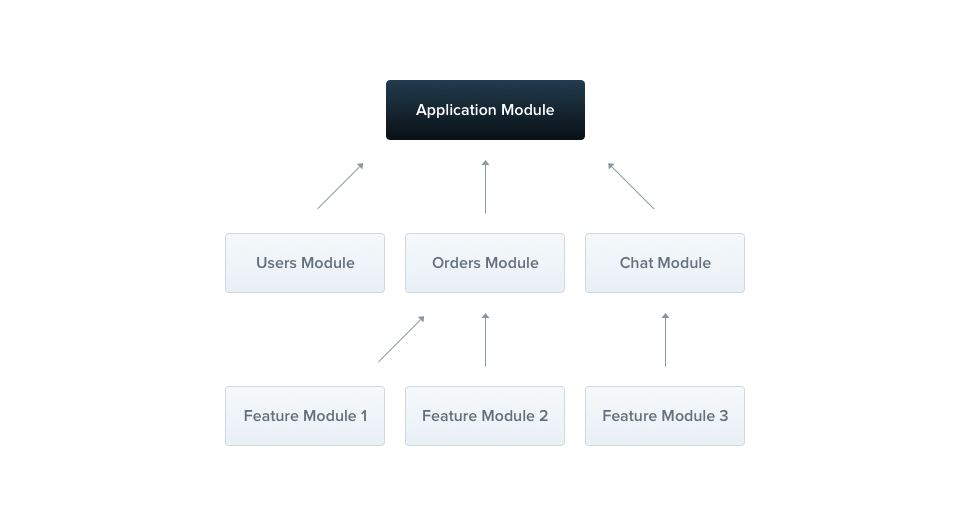
\includegraphics[width=1\textwidth]{Images/technology/module-nestjs.png}
        \caption{NestJS được tổ chức thành các đơn vị gọi là module}
    \end{figure}
Một trong những điểm quan trọng khi áp dụng NestJS vào dự án là sự xuất hiện của 3 khái niệm Modules, Controllers và Services
\begin{itemize}
    \item \textbf{Module}: Ứng dụng dựa trên nền tảng NestJS được xây dựng bằng các modules. Modules là các containers chứac các thành phần khác nhau của ứng dụng như services, controllers và các components có liên quan. Module có chức năng quản lý và đóng gói các tính năng của ứng dụng. Một module có thể là một tính năng hoặc một phần của ứng dụng. Ví dụ như có thể tồn tại các module về xác thực (authentication) , quản lý người dùng (user management), hoặc quản lý sản phẩm. Mục đích của cách tiếp cận này là dễ dàng quản lý các tính năng và đem lại sự tiện lợi trong việc nâng cấp và bảo trì ứng dụng.

    \item \textbf{Controllers}: có tác dụng xử lý các yêu cầu HTTP và đưa ra các response, phục vụ các entry point về phần logic của ứng dụng. Mỗi một controller sẽ gắn với một route cụ thể hoặc một endpoint mà ở đó được định nghĩa các function để xử lý các yêu cầu. Controllers sử dụng các decorators để tương tác với các route path bằng các phương thức HTTP bao gồm (GET, POST, PUT, DELETE,...) và các parameters. Các controller cũng có thể tương tác với service để thực hiện các business logic.
    \begin{figure}[H]
        \centering
        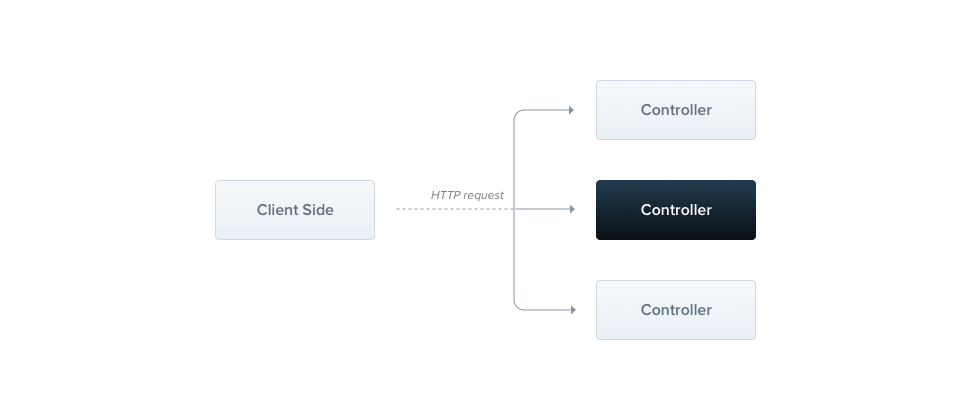
\includegraphics[width=1\textwidth]{Images/technology/controller_2.png}
        \caption{Controller của NestJS xử lý các endpoint được gọi từ phía client}
    \end{figure}
    \begin{figure}[H]
        \centering
        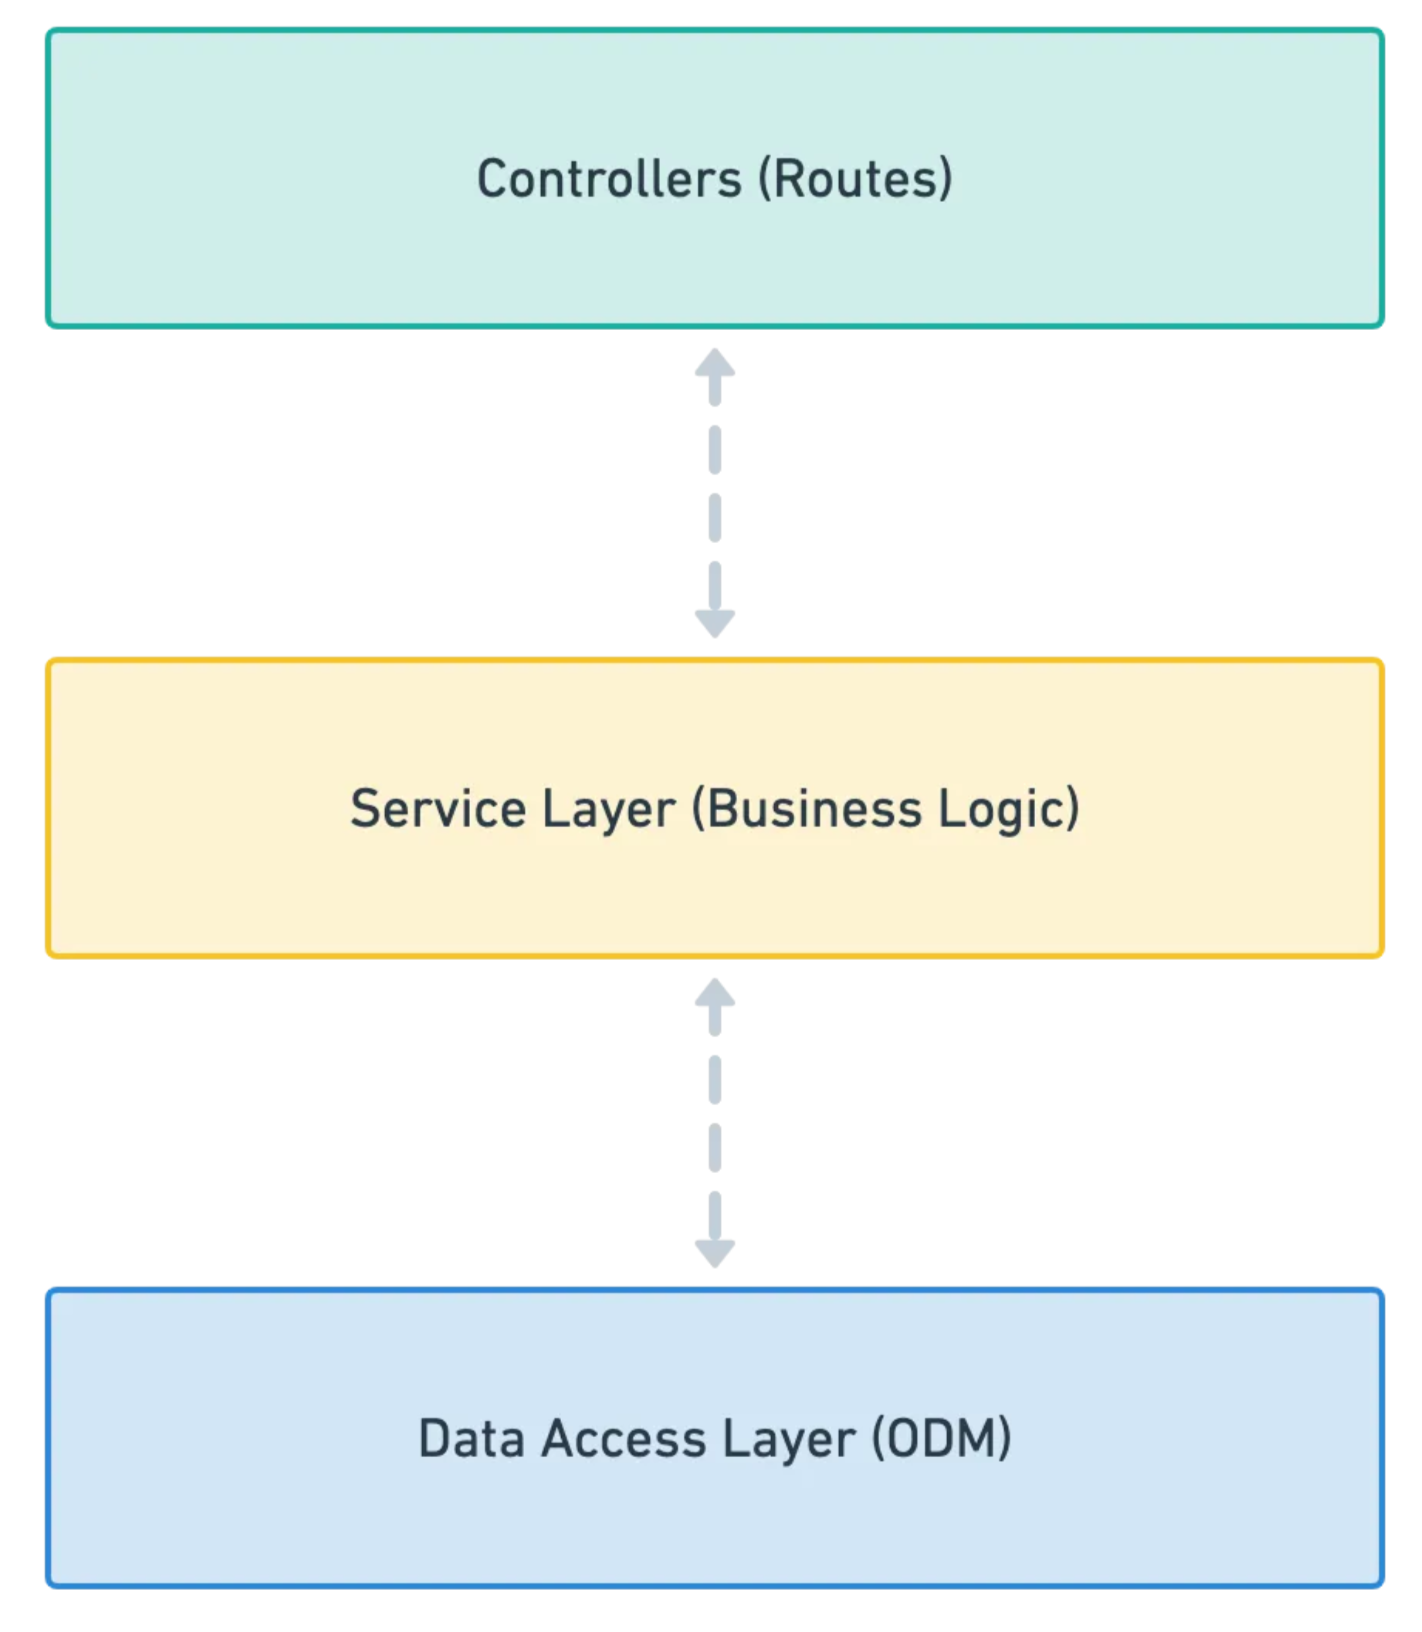
\includegraphics[width=0.4\textwidth]{Images/technology/controller.png}
        \caption{Các layer trong một ứng dụng NestJS}
    \end{figure}
    
    \item \textbf{Services}: có chức năng để định nghĩa các hàm xử lý các logic và data trong một dự án sử dụng NestJS. Service đóng gói các business logic và các hàm để xử lý data, sau đó các hàm trên sẽ được gọi trong controllers để thực hiện các chức năng như lấy dữ liệu từ database, tương tác với API hoặc xử lý các tính năng liên quan đến data. Service đóng vai trò như một chức năng của úng dụng khi mà controllers được dùng để xử lý các yêu cầu được gửi đến và đi. Service thường được sử dụng trực tiếp tại controllers mà ở NestJS được miêu tả với một từ rất đặc trưng \textbf{Injectable} tại file service để giúp dễ dàng quản lý các dependencies và nâng cao khả năng kiểm thử.
\end{itemize}
\subsubsection{Các tính năng nổi bật}
Các tính năng nổi bật của NestJS bao gồm:
\begin{itemize}
    \item Kiến trúc theo module: NestJS phát triển kiến trúc theo module để lập trình viên tiện trong việc quản lý dự án theo module, components, services và các controllers. Mục đích của việc này là nhằm tối ưu dự án để dễ nâng cấp và bảo trì
    \item Được tối ưu cho Typescript do vậy NestJS đem đến cho người dùng các lợi ích về codebase cũng như khả năng tìm ra lỗi, debug nhanh hơn
    \item Module microservices của NestJS hỗ trợ đủ loại kết nối: RabbitMQ, gRPC, Kafka, Redis,...
    \item Middleware và Guard được tích hợp trong NestJS, với vai trò để thực hiện các task như authentication, logging, hoặc data validation.
    \item Exception Handling: NestJS cung cấp một cơ chế xử lý exception dễ dàng, cho phép quản lý và xử lý các ngoại lệ trong ứng dụng.
    \item WebSocket: NestJS hỗ trợ WebSocket, cho phép xử lý kết nối realtime giữa client và server.
\end{itemize}
\subsubsection{Phân tích ưu và nhược điểm}
\textbf{Ưu điểm}
\begin{itemize}
    \item Khả năng mở rộng và bảo trì tốt do được xây dựng trên kiến trúc module, và đồng thời quản lý code được dễ dàng hơn
    \item Testing được cung cấp các dependencies để sử dụng khi viết unit test, integration test hoặc end to end test được gọn gàng hơn
    \item Tích hợp được với nhiều thư viện, kết hợp tốt với các tool và framework, ngoài ra có một số lượng lớn người sử dụng nên sẽ hiệu quả trong việc sửa lỗi khi gặp vấn đề
\end{itemize}
\textbf{Nhược điểm}
\begin{itemize}
    \item Không thích hợp với các dự án nhỏ do quá trình setup khá phức tạp, tốn rất nhiều công sức
    \item Cộng đồng chỉ đang phát triển chưa thực sự quá lớn mạnh.
    \item Kiến trúc được lấy cảm hứng từ Angular do vậy sẽ gặp khó khăn nếu như chưa từng làm qua Angular
\end{itemize}
\subsection{PostgreSQL}
\subsubsection{Tổng quan}
PostgreSQL là một hệ quản lý cơ sở dữ liệu được dùng khá phổ biến và được biết đến với nhiều tính năng tốt, khả năng mở rộng tốt cũng như cách quản lý mã nguồn hiệu quả
\subsubsection{Các tính năng nổi bật}
PostgreSQL là một trong những hệ quản trị cơ sở dữ liệu quan hệ phổ biến nhất và được sử
dụng rộng rãi trên thế giới. Nó được ưa chuộng bởi: 
\begin{itemize}
    \item PostgreSQL cung cấp khả năng bảo mật tốt, khả năng chịu đựng lỗi cao mà không ảnh hưởng đến các phần khác 
    \item Có khả năng mở rộng cao cả về số lượng dữ liệu và số lượng người dùng có thể thao tác cùng lúc
    \item Truy vấn nhanh chóng và bảo mật duy trì tính toàn vẹn và độ tin cậy. Để đáng tin cậy hơn
    \item Khả năng tương thích đa nền tảng, khả năng đồng thời xử lý nhiều kết nối, hiệu suất cao và khả năng xử lý dữ liệu lớn.
\end{itemize}
\subsubsection{Phân tích ưu và nhược điểm}
\textbf{Ưu điểm}
\begin{itemize}
    \item PostgreSQL được đánh giá là một trong những hệ quản trị cơ sở dữ liệu có độ tin tưởng cũng như bảo mật cao
    \item PostgreSQL cũng được trang bị nhiều tính năng để xử lý với một số lượng data khổng lồ
    \item Được sử dụng để chạy trang web và ứng dụng web động.
    \item Cho phép lưu lại nhật ký và hình thành cơ sở dữ liệu hỗ trợ sửa lỗi.
\end{itemize}
\textbf{Nhược điểm}
\begin{itemize}
    \item Một số extension không được hỗ trợ trên cloud do vậy phải mất thời gian đề cấu hình chỉnh sửa theo ý muốn
    \item Không hỗ trợ real-time data trong một vài trường hợp cần real-time retrieval
    \item Hiệu suất hoạt động thực tế chậm hơn so với MySQL
    \item Nhiều ứng dụng nguồn mở chỉ hỗ trợ MySQL và không hỗ trợ PostgreSQL
\end{itemize} 
\subsection{Prisma}
\subsubsection{Tổng quan}
\hspace*{1cm} Prisma là một ORM (Object-Relational Mapping) được thiết kế để làm cho việc truy cập cơ sở dữ liệu dễ dàng hơn trong các ứng dụng Node.js và TypeScript. Nó cung cấp một API dễ sử dụng để truy cập cơ sở dữ liệu mà không cần phải viết các câu lệnh SQL trực tiếp. Prisma tự động tạo ra các bảng cơ sở dữ liệu và cập nhật cấu trúc khi thay đổi mô hình dữ liệu. Prisma hỗ trợ nhiều loại cơ sở dữ liệu như PostgreSQL, MySQL và SQLite. Trong đó ORM(object relational Mapping) là một kỹ thuật giúp chuyển các đoạn mã lưu trữ dữ liệu dưới dạng OOP(Object Oriented Programming) sang relational database \cite{prisma}.\\
\begin{figure}[H]
    \centering
    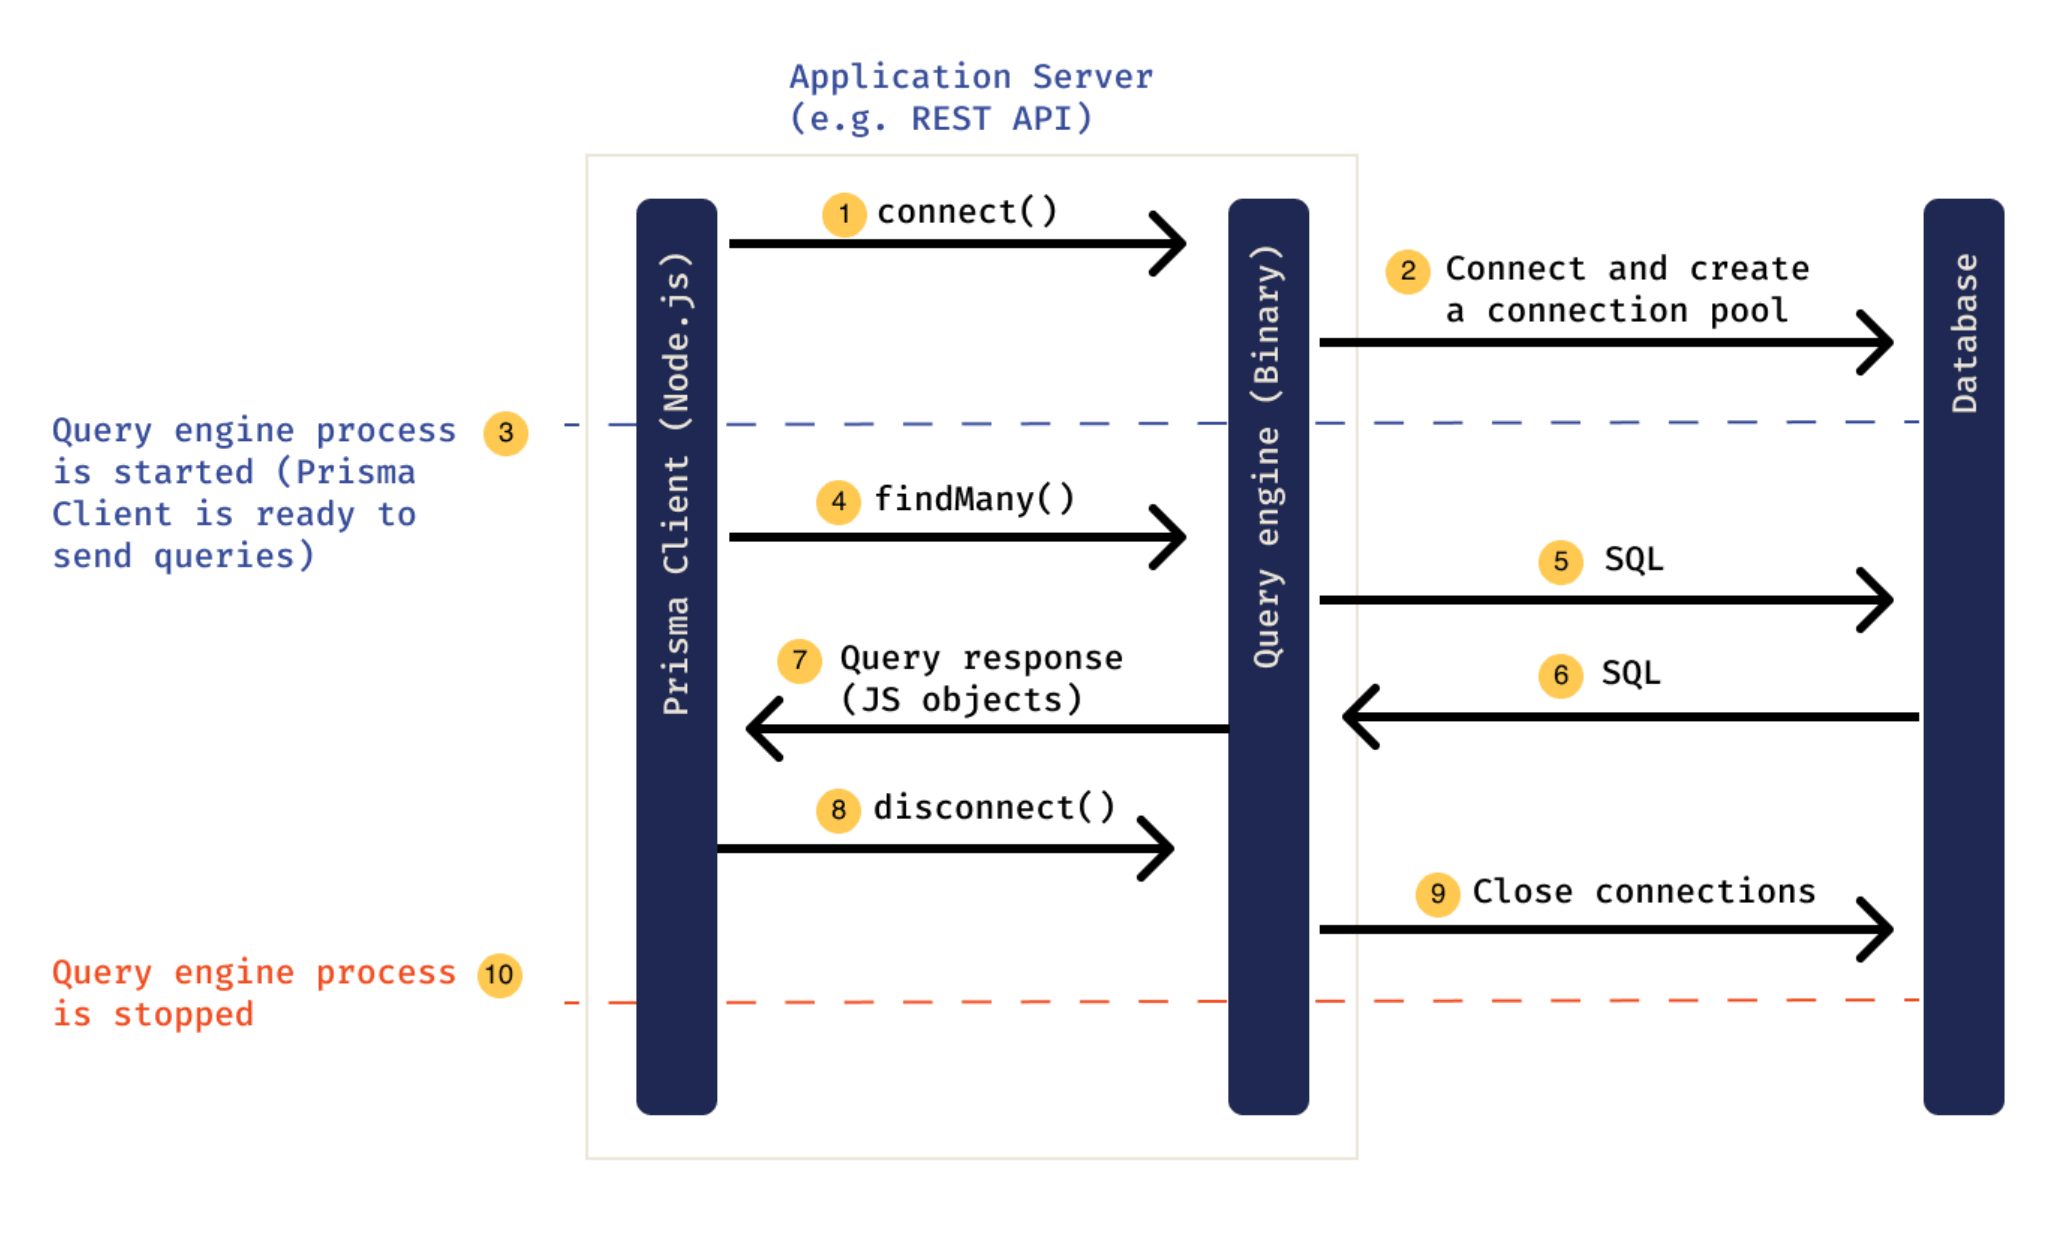
\includegraphics[width=0.9\textwidth]{Images/technology/prisma-architecture.png}
    \caption{Prisma cung cấp các phương thức để ứng dụng có thể tương tác với database}
\end{figure}
\textbf{Cách thức hoạt động của Prisma:}
\begin{enumerate}
    \item Prisma sử dụng những model được viết dưới dạng schema và lưu trữ ở client và tạo kết nối với Query Engine
    \item Tạo kết nối từ Query Engine và Database
    \item Truyền một lệnh query để truy xuất dữ liệu chuyển nó thành lệnh SQL trong Database
    \item Chờ dữ liệu gửi về từ Database
    \item Ngắt kết nối
\end{enumerate}
Prisma cung cấp một API đơn giản và dễ sử dụng để thao tác với cơ sở dữ liệu, cho phép
bạn thực hiện các thao tác CRUD (Create, Read, Update, Delete) một cách nhanh chóng và dễ
dàng.
\subsubsection{Các tính năng nổi bật}
Prisma bao gồm ba phần chính:
\begin{itemize}
    \item Prisma Client : Trình tạo truy vấn an toàn và được tạo tự động cho Node.js và TypeScript.
    \item Prisma Migrate : Hệ thống dùng để di chuyển và mô hình hóa dữ liệu.
    \item Prisma Studio : GUI để xem và chỉnh sửa dữ liệu trong cơ sở dữ liệu.
\end{itemize}
\subsubsection{Phân tích ưu và nhược điểm}
\textbf{Ưu điểm}
\begin{itemize}
    \item Prisma có khả năng mở rộng và tái sử dụng, cho phép bạn tạo ra các ứng dụng phức tạp và có thể mở rộng dễ dàng. 
    \item Prisma hỗ trợ các tính năng như transacations, batching và lazy-loading, giúp tối ưu hóa hiệu suất và giảm thiểu số lần truy cập cơ sở dữ liệu.
    \item Bên cạnh đó, Prisma cũng cho phép định nghĩa các ràng buộc duy nhất, khóa ngoại và các mối quan hệ giữa các bảng. Prisma tự động sinh ra mã TypeScript cho các truy vấn cơ sở dữ liệu, giúp bạn phát hiện lỗi trước khi thực thi chương trình.
\end{itemize}
\textbf{Nhược điểm}
\begin{itemize}
    \item Cộng đồng còn nhỏ, sẽ gặp khó khăn khi gặp vấn đề do không có nhiều người hỗ trợ
    \item Tuy Prisma cung cấp một lớp trừu tượng nhằm tăng hiệu suất và các lệnh để tương tác với database, nhưng một vài dự án đòi hỏi những lệnh query phức tạp thì chưa thể đáp ứng
\end{itemize}
\subsection{JWT}
\subsubsection{Tổng quan}
JSON Web Token (JWT) \cite{jwt} là một tiêu chuẩn mở định nghĩa một cách ngắn gọn và khép
kín để truyền dẫn thông tin giữa hai bên client và server được định dạng bằng JSON.
Chuỗi JWT gồm 3 thành phần là header, payload, signature và được ngăn cách nhau bằng
dấu chấm (“.”).
\begin{figure}[H]
    \centering
    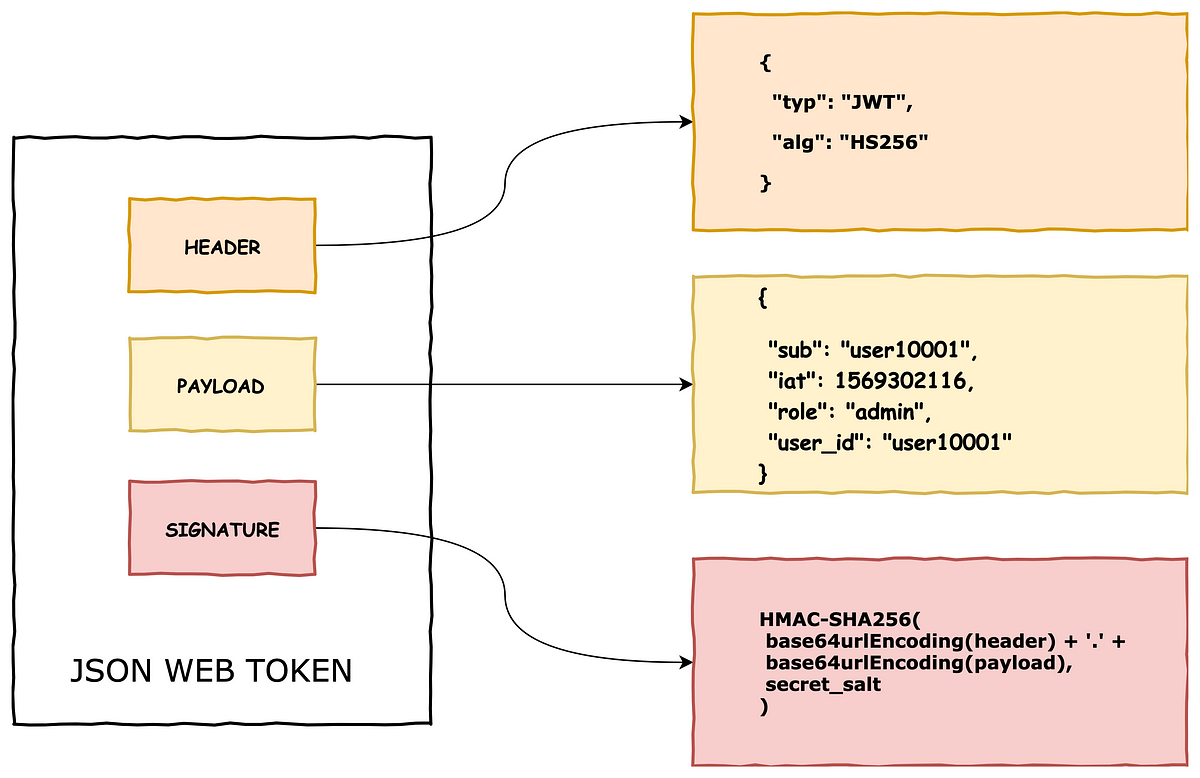
\includegraphics[width=0.7\textwidth]{Images/technology/jwt_structure.png}
    \caption{Cấu trúc của JSON web token}
\end{figure}
\begin{itemize}
    \item \textbf{Header}: Phần header thường chứa hai phần là kiểu dữ liệu (giá trị thường là JWT) và thuật toán sử dụng để mã hóa chuỗi như HMAC SHA256 hoặc RSA
    \item \textbf{Payload}: Phần payload chứa thông tin muốn đặt trong chuỗi ví dụ như tên đăng nhập (username), id của người dùng (user id), tên người dùng,...Phần payload sẽ được mã hóa Base64Url tạo thành phần thứ hai của chuỗi JWT.
    \item \textbf{Signature}: Phần signature này sẽ được tạo ra bằng cách mã hóa phần header và phần payload kèm theo một chuỗi secret (khóa bí mật)
\end{itemize}
\textbf{Quy trình của xác thực client với JWT}:
\begin{enumerate}
    \item Người dùng sẽ gửi thống tin xác thực của mình đến server xác thực.
    \item Server sẽ kiểm tra thông tin người dùng cung cấp có đúng không. Nếu dúng thì chuyển sang bước tiếp theo, ngược lại thì trả lỗi về cho người dùng.
    \item Server xác thực sẽ thực hiện ký lên thông tin của người dùng kèm với một số claims khác như thời gian cấp, thời điểm hết hạn và thời điểm mà token bắt đầu trở nên hợp lệ.
    \item Sau khi người dùng nhận được token, họ sẽ đính kèm token này vào các lời gọi API (thường là bỏ ở header Authorization của api request).
    \item Server xử lý các api request sẽ tiến hành parse token và xử lý xác thực để cho phép người dùng truy cập các resource
\end{enumerate}
\begin{figure}[H]
    \centering
    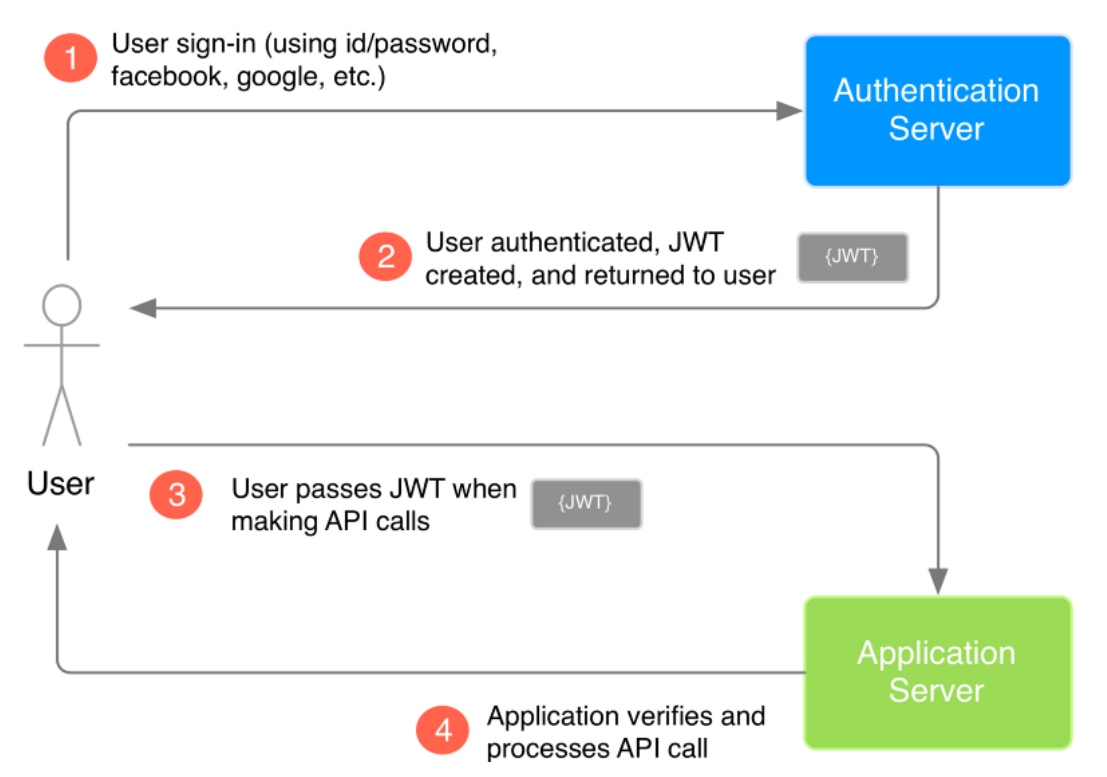
\includegraphics[width=0.7\textwidth]{Images/technology/jwt authentication.png}
    \caption{Quy trình xác thực client với JWT}
\end{figure}
\subsubsection{Các tính năng nổi bật}
\begin{itemize}
    \item \textbf{Xác thực (Authentication)}: Đây là trường hợp phổ biến nhất sử dụng JWT. Sau khi người dùng đăng nhập vào hệ thống, thì những request tiếp theo từ phía người dùng sẽ chứa thêm mã JWT. Điều này cho phép người dùng có quyền truy cập vào các url, service, và resource mà mã Token đó cho phép.
    \item \textbf{Trao đổi thông tin}: JWT là 1 cách khá hay để truyền thông tin an toàn giữa các thành viên với nhau. Và nhờ vào phần signature của nó, phía người nhận có thể biết được người gửi là ai thông qua phần signature. Và chữ ký được tạo ra bằng việc kết hợp cả phần header và phần payload lại nên thông qua đó ta có thể xác nhận được chữ ký đó có bị giả mạo hay không.
\end{itemize}

\subsubsection{Phân tích ưu và nhược điểm}
\textbf{Ưu điểm}
\begin{itemize}
    \item Đơn giản, gọn nhẹ: Như ta có thể thấy ở trên, việc xác thực với JWT vô cùng đơn giản và gọn nhẹ. Việc lưu trữ token hoàn toàn nằm ở phía client giúp phần nào giảm tải được nhu cầu về tài nguyên lưu trữ và tính toán ở server. Đây là một ưu điểm nổi bật khi so sánh với các phương pháp truyền thống khác sử dụng Session hay Cookies.
    \item Dễ lập trình: JWT được hỗ trợ và sử dụng rộng rãi nên hầu như tất cả ngôn ngữ lập trình backend đều hỗ trợ việc tạo và xác thực các JWT một cách tiện lợi.
    \item Dễ scale: việc xác thực với JWT không yêu cầu lưu trữ thêm thông tin ở phía server, ứng dụng của ta có thể scale tốt hơn mà không phải tốn thêm quá nhiều chi phí cho các server và database xác thực người dùng.
\end{itemize}
\textbf{Nhược điểm}
\begin{itemize}
    \item  Vì JWT token nằm hoàn toàn ở phía client nên ta không thể hủy các token một cách chủ động từ backend. Để chống một số loại tấn công DOS ta phải ràng buộc thời hạn hợp lệ của token và hiện thực thêm các cơ chế cấp lại token mới cho người dùng.
\end{itemize}